%!TEX root = main.tex
\section{Introduction}% 

\par 
With the ever-increasing complexity 
and size of datasets,
there is a growing demand for 
information visualization tools
that can help data scientists make sense of large
volumes of data.
Visualizations help discover 
trends and patterns, 
spot outliers and anomalies, 
and generate or verify hypotheses.
Moreover, 
visualizations are visceral and intuitive: 
they tell us stories about our data; 
they educate, delight, inform, 
enthrall, amaze, and clarify.
This has led to the overwhelming popularity
of point-and-click visualization tools like Tableau~\cite{Stolte2002},
as well as programmatic toolkits like ggplot, D3, Vega, and matplotlib. 
We term these tools as {\em visualization-at-a-time} approaches, since
data scientists need to individually 
generate each visualization (via code or interactions),
and examine them, 
one at a time.


\par
As datasets grow in size and complexity, 
these visualization-at-a-time approaches start to break down,
due to the limited time availability on the 
part of the data scientists---there 
are often too many visualizations to examine for a given 
task, such as identifying outliers, or inferring patterns. 
Even on a single table, 
visualizations can be generated
by varying the subsets of data operated on, 
or the attributes (or combinations
thereof) that can be visualized. 
If we add in various visualization modalities, encodings,
aesthetics, binning methods, and transformations,
this space becomes even larger.


\par
Thus, there is a pressing need for an 
intelligent,
interactive, understandable, usable, and
enjoyable tool that can help 
data scientists navigate
collections of visualizations.
We term our hypothesized tool \vida,
short for {\em VIsual Discovery Assistant}.
Data scientists specify their discovery
goal at a high level,
with \vida 
automatically 
traversing visualizations to provide
solutions or partial solutions for the
specified discovery goal, thereby
eliminating the tedium and wasted
labor of comparable visualization-at-a-time 
approaches.

\par
\stitle{\vida Dimensions.} In order to be a holistic solution for 
navigating collections of visualizations,
\vida must be able to support various discovery
settings. 
We organize these settings along two
dimensions, displayed along the columns and rows (respectively) of Table~\ref{fig:table}---first, the overall discovery goal,
and second, the degree of specificity of the goal.
We also cite references (described later on)
for systems that partially provide the necessary
functionality for the given setting.

\par
 We identify five 
common discovery goals in visual data exploration, organized
along the columns:
{\em finding patterns}, {\em identifying anomalies/clusters}, {\em summarizing}, 
{\em performing comparisons}, {\em providing explanations}.
These five goals borrow borrow from functionalities in existing
systems, as well as related visualization task taxonomies~\cite{Heer2012,Amar2005}.
We omit low-level goals such as filtering or sorting, since
these functionalities are common in 
visualization-at-a-time tools and toolkits.
We also omit goals that go beyond visual data exploration,
such as extrapolation, supervised learning, and cleaning, among others. 

\par 
 We identify three degrees of specificity
for the discovery goal, organized along the rows:
{\em precise}, {\em fuzzy}, {\em underspecified}.
The degree of specificity characterizes the division
of work between how much user has to specify
versus how much the system has to automatically
infer and aid in accomplishing the discovery goal. 
At the topmost row, the onus is placed on the user
to provide an exact and complete specification of 
what the solution to their discovery
goal must look like;
at the middle row, the user can provide
a vague specification of what the solution must look like;
and finally, at the bottom row,
the user provides a minimal specification, or
leaves the characteristics of the solution underspecified,
leaving it up to the system to ``fill in'' the rest.
Naturally, as we proceed down the rows,
it gets harder for the system to automatically
interpret what the user might have in mind as a solution
to their discovery goal.

\begin{table}[!t]
\scriptsize
\centering
\begin{tabular}{l|l|l|l|l|l}
& \multicolumn{5}{c}{Discovery Goals}                                                                     \\ \hline
& Find Patterns & Identify Anomalies and Clusters      & Compare           & Summarize  & Explain          \\ \hline
Precise (Section~\ref{sec:precise}) & \multicolumn{3}{c|}{Zenvisage~\cite{Lee2017}, ZQL~\cite{Siddiqui2016}}                                      &            &                  \\ \hline
Fuzzy (Section~\ref{sec:vague})     & ShapeSearch\cite{Siddiqui2018}   & Scorpion\cite{Wu2013}, Profiler~\cite{Kandel2012}, Natural Language & Natural Language~\cite{Fast2018,Setlur2016,Hoque2017}  &            & Natural Language \\ \hline
Minimal (Section~\ref{sec:minimal}) &               & \multicolumn{1}{c|}{Storyboard~\cite{Lee2018}}      & SeeDB~\cite{Vartak2015}, Storyboard & Storyboard & Storyboard      
\end{tabular}
\caption{Overview of the systems described in this paper. Columns are organized into discovery goals and rows are ordered by decreasing levels of query specificity and correspondingly increasing levels of autonomous assistance.}\label{fig:table}
\end{table}

\par
\stitle{\vida Input Modalities.} To support the spectrum of 
demands imposed by the
discovery settings described above, \vida 
must support a range of interactive input modalities,
as displayed in Figure~\ref{fig:cycle},
catering to a range of user expertise and preferences.
These input modalities include 
\begin{itemize}
	\item natural language, via a keyword search box, or a dialog or conversational interface;
	\item interactions, either with an existing visualization, such as brushing-and-linking or hovering, or those that construct a new one, such as drag-and-drop or sketching; and
	\item restricted template queries, involving selection of operations and operands from a drop-down menu.
\end{itemize}
We will provide examples of these input modalities in subsequent sections.
Each of these inputs are compiled down
into a query in a query language, called \vidaql.
Alternatively, expert users may directly invoke \vidaql queries.
\vidaql queries will natively support the five discovery goals,
and will also support combinations thereof, e.g., pattern search followed by 
summarization. 
Another important element is how much does a user actively ``request'' (pull)
versus \vida ``recommending'' visualizations (push). 
Given that we expect \vida to support a range of specificities,
\vida must support both push and pull, with pull decreasing
in importance, and push rising in importance, as we go from precise to minimal.

\begin{figure}[h!]
\label{fig:cycle}
\centering
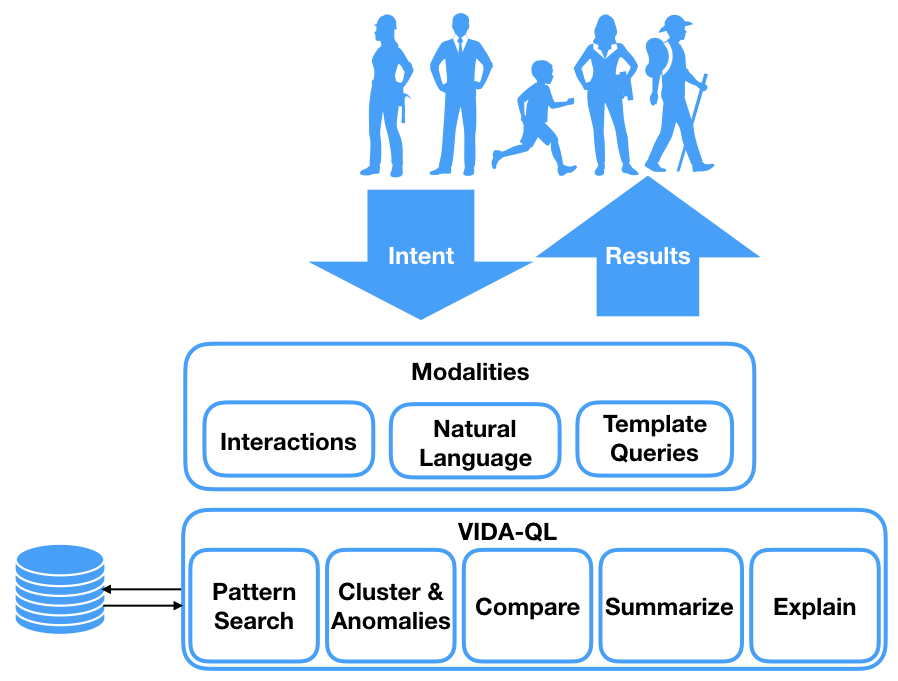
\includegraphics[width=0.5\linewidth]{figures/VIDA_architecture.png}
\caption{\vida Architecture\agp{fix; convert figure into a wrapfigure}}
\end{figure}


% Common framework and module means there are underlying functionalities can be shared (e.g. statistical modules, data heavy-lifting operations)
% - From the top: many different types of users (novices/experts), each with some high-level intent in one of the following modalities:
%      - Interaction: produces as an output either through the creation a visualization (e.g. sketching, drag-and-drop) or changes upon a visualization (e.g. brushing, selections, clicks)
%      - Partial specification includes some minimal input such as input X,Y of interest
%      - Either that or user can directly specify their query exactly in VIDA-QL
% - VIDA-QL contains 5 discovery modules which each have their own "push and pull" components, i.e. work with both search and recommend.

\par
\stitle{Outline.}
The rest of our paper is organized along the degree of specificity
of discovery goal, and we will allude to the specific discovery
goals as well as input modalities as we go along. 
The degree of specificity of the discovery goal is the factor
that most significantly affects the architecture of \vida,
with the complexity increasing as the specificity decreases. 

\par In Section~\ref{sec:precise}, we discuss the 
the {\em precise} setting.
Our tool, \zv, is an example of a solution for
this setting, partially eliminating the problem
of having to manually examine large numbers 
of visualizations in search of a desired pattern, 
which can be error-prone and inefficient. 
Our \zv design study demonstrates
that precise setting is insufficient for
addressing all of the demands of real-world use-cases.
\agp{got until here.}


In addition, we find that users often do not have a good idea of what they want to query for without looking at example visualizations or summaries of the data. To bridge the gap between user's high-level intent and what the system operates as inputs, we advocate that future research needs to look beyond simple precise visual querying by : 1) making visual query system more expressive by supporting a wider class of vague queries (Section~\ref{sec:vague}) and 2) making it easier to know what to query by recommending visualizations that facilitate data awareness (Section~\ref{sec:minimal}).
\par Accordingly, the next row in the table highlights a growing class of \textit{intelligent visual querying system} (IVQS) that interprets the `vagueness' of queries and allow users to tweak or refine their queries through a feedback mechanism. \dor{I think we need to expand this definition depending on the new content that we will be adding, ShapeSearch, SeeDB, Scorpion?} 
\par To address the problem of guiding users to portions of the data that they might be interested in querying, Section~\ref{sec:minimal} introduces systems that help users become more aware of their dataset and visualize where they are in their analysis workflow. The challenge in building these systems involves understanding what types of visualizations should be recommended to facilitate data awareness. As an example, we describe our work on \sbd, a system that provides data summaries and guides users through informative subsets of data. Finally, we discuss related works on how visualizing provenance and situational information can guide users towards more informative analysis actions.